%!TEX root = foglio.tex

Quantili: $q_\alpha$ è tc $\PP(X\leq q_\alpha)=\alpha$, analogamente $q_{1-\alpha}$ è tc $\PP(X>q_{1-\alpha})=\alpha$

\smallskip

% =================================================

\section{Stat s-m-c}

% =================================================

\subsection{Stat sufficienti}

Def di stat: è una funz del campione, cioè $T(\mathbf{X})$ 

\smallskip

Def di suff: $T(\mathbf{X})$ è stat suff se la legge di $\mathbf{X}|T=t$ non dipende da $\theta$ per ogni $t$ 

\smallskip

Principio di stat suff: $T(\mathbf{X})$ è suff per $\theta$ quando ogni inferenza su $\theta$ dip da $\mathbf{X}$ solo tramite $T(\mathbf{X})$

\smallskip

Criterio di fatt: una stat  $T(\mathbf{X})$ è suff per $\theta$ \textit{sse} $\exists g, h$ tc $f(\mathbf{x},\theta)=h(\mathbf{x})\cdot g(T(\mathbf{x}),\theta)$

\begin{proof}
(caso discreto, senza perdita di generalità) Per ipotesi, $T(\mathbf{X})$ è stat suff. Preso $T(\mathbf{x})=t$:
\begin{align*}
f(\xv,\theta)&=\PP_\theta(\Xv=\xv) \\
&=\PP_{\xcancel{\theta}}(\Xv=\xv|T(\Xv)=t)\cdot \PP_\theta(T(\Xv)=t) \\
&=h(\mathbf{x})\cdot g(t,\theta)\ \Rightarrow\ \text{vale fatt}
\end{align*}
Ora per ipotesi vale la fatt. Prese $q(t,\theta)$ la densità di $T$ e $A_T=\{\yv\text{ tc }T(\yv)=T(\xv)\}$, la legge di $\Yv|T(\xv)$ è
\begin{gather*}
\frac{f(\xv,\theta)}{q(T(\xv),\theta)}=\frac{g(T(\mathbf{x}),\theta) \cdot h(\xv)}{\sum_{\yv\in A} g(T(\mathbf{y}),\theta) \cdot h(\yv)}= \\
=\frac{\cancel{g(T(\mathbf{x}),\theta)} \cdot h(\xv)}{\cancel{g(T(\mathbf{y}),\theta)} \sum_{\yv\in A} h(\yv)}=\frac{h(\xv)}{\sum_{\yv\in A} h(\yv)}\\
\text{che non dip da }\theta\ \Rightarrow\ \text{stat suff}\qquad \blacksquare
\end{gather*}
\end{proof}

Cor: date $T(\mathbf{X})$ stat suff e $r(\cdot)$ funz biunivoca, $T^*(\mathbf{X})=r(T(\mathbf{X}))$ è stat suff

\begin{proof}
Dato che $T(\mathbf{X})$ è stat suff, per il criterio di fatt posso scrivere:
\begin{align*}
f(\mathbf{x},\theta)&=h(\mathbf{x}) \cdot g(T(\mathbf{x}),\theta) \\
&=h(\mathbf{x}) \cdot g(r^{-1}(T(\mathbf{x})),\theta) \\
&=h(\mathbf{x}) \cdot g^*(T^*(\mathbf{x}),\theta) \ \Rightarrow\ T^* \text{ stat suff}\quad\blacksquare
\end{align*}
\end{proof}

\subsection{Stat (sufficienti e) minimali}

Def di stat suff e min: $T(\Xv)$ è s-m se è funzione di ogni altra stat suff

\smallskip

Teo di LS1: $T(\Xv)$ è stat s-m per $\theta$ se
\begin{equation*}
\frac{f(\xv,\theta)}{f(\yv,\theta)}\text{ non dip da }\theta\ \Leftrightarrow\ T(\xv)=T(\yv)\quad \forall \xv,\yv
\end{equation*}

\subsection{Stat complete}

Def: detta $h(t,\theta)$ la famiglia di densità per la stat $T(\Xv)$, diciamo che $h$ è completa (cioè $T$ stat completa) se $\forall g$ misurabile e $\forall \theta$ vale che $\EE_\theta\left[g(T)\right]=0$ $\Rightarrow$ $g(T)=0$ qo 

\smallskip

Teo di Bahadur: suff compl $\Rightarrow$ min 

\subsection{Exponential Family}

$f(x,\underline{\theta})=h(x)\cdot c(\underline{\theta})\cdot \text{exp}\left\{\sum_{i=1}^k w_i(\underline{\theta})\ t_i(x)\right\}$

\smallskip

Trovare stat s-m-c nella EF: $T(\xv)=\left(\sum_{i=1}^n t_1(x_i),\dots,\sum_{i=1}^n t_k(x_i)\right)$ è suff, è anche compl se $\left(w_1(\underline{\theta}),\dots,w_k(\underline{\theta})\right)$ mappa $\Theta$ in un insieme che contiene almeno un aperto di $\RR^k$, è anche min per Bahadur

\subsection{Stat ancillari}

Def: stat S la cui $f$ non dip da $\theta$ (S $\Bot$ s-m-c)

% =================================================

\section{Stimatori}

% =================================================

Def di stimatore puntuale per $\theta$: è una qualunque funz solo di $\Xv$  

\subsection{Metodo dei momenti}

Uguaglio momenti teorici $\EE\left[X_i^k\right]$ a momenti empirici $\frac{1}{n}\sum_{i=1}^n X_i^k$ (stime fornite non sempre ammissibili, cioè $\notin \Theta$)

\subsection{Stimatori di max verosimiglianza}

Def: $\hat{\theta}_{\text{MLE}}(\xv)=\text{ArgSup}_{\theta\in\Theta} L(\xv,\theta)$ (stime sempre ammissibili)

\smallskip

Principio di invarianza per MLE: lo stimatore MLE di $\tau(\theta)$ è $\tau\left(\hat{\theta}_{\text{MLE}}\right)$

\subsection{MSE}

$\text{MSE}(T)=\EE[(T-\theta)^2]=\text{Var}(T)+\left(\EE[T]-\theta\right)^2$

\smallskip

Stimatore corretto/non distorto: se $\EE_\theta[T]=0$

\subsection{UMVUE e Cramer-Rao}

Def: $\widetilde{T}$ è UMVUE per $\theta$ se $\widetilde{T}$ è lo stimatore non distorto di $\theta$ a varianza/MSE minima/o 

\smallskip

Dis. di Cramer-Rao: siano $X_i\overset{iid}{\sim} f(x,\theta)$ e sia $T(\Xv)$ stimatore di $\theta$; se \\
$\begin{array}{l}
(1)\ \text{supp}(X_i)\text{ non dip da }\theta \\
(2)\ \EE_\theta\left[T^2\right]<\infty \\
(3)\ \frac{\de}{\de\theta}\EE_\theta[T]=\int_{\RR^n} T(\xv)\ \frac{\partial}{\partial \theta}\,f(\xv,\theta)\,\de\xv
\end{array}$ \\
allora $\text{Var}_\theta(T)\geq l_{CR}=(\frac{\de}{\de\theta}\EE_\theta[T])^2/I_n(\theta)$, dove $I_n(\theta)=\EE_\theta\left[\left(\frac{\partial}{\partial\theta}\,\log\,f(\xv,\theta)\right)^2\right]$ è l'info di Fisher

\begin{proof}
Siano $X=T$ e $Y=\frac{\partial}{\partial\theta}\,\log\,f(\xv,\theta)$.

Passo I $\rightarrow$ scrivo l'ip (3) per $T(\xv)=1$:
$\begin{array}{l}
0=\frac{\de}{\de\theta}\EE[1]=\int_{\RR^n} \frac{\partial}{\partial\theta} \left[f(\xv,\theta)\right]\dxv \\
=\left\{\circledast:\frac{\partial}{\partial\theta}\left(\log\,f\right)=\frac{1}{f}\cdot f'   \right\} \\
=\int_{\RR^n} \frac{\partial}{\partial\theta} \left[\log f(\xv,\theta)\right] f(\xv,\theta)\dxv = \EE[Y]
\end{array}$

Passo II $\rightarrow$ calcolo il numeratore:
\begin{align*}
\frac{\de}{\de\theta}\EE[T]&\overset{(3)}{=}\int_{\RR^n}T(\xv)\,\frac{\partial}{\partial\theta}f(\xv,\theta)\dxv \\
&\overset{\circledast}{=}\int_{\RR^n}T(\xv) \frac{\partial}{\partial\theta} \left[\log f(\xv,\theta)\right] f(\xv,\theta)\dxv \\
&=\EE[T\cdot Y]\overset{\text{I}}{=}\Cov(X,Y)
\end{align*}

Passo III $\rightarrow$ calcolo il denominatore: \\
$I_n(\theta)=\left[\left(\frac{\partial}{\partial\theta}\,\log\,f(\xv,\theta)\right)^2\right]=\EE\left[Y^2\right]\overset{\text{I}}{=}\Var(Y)$

Sostituendo II e III nella disuguaglianza di CS: \\
$\Var(X)\geq\frac{|\Cov(X,Y)|^2}{\Var(Y)} \leadsto \text{tesi}\qquad\blacksquare$
\end{proof}

\subsection{Parentesi sull'info di Fisher}

Lemma 1: sotto le hp della dis. di CR (che valgono sempre se $\in$EF) vale che $I_n(\theta)=nI_1(\theta)$ (densità unimodale)

\begin{proof}$\\$
$\begin{array}{l}
I_n(\theta)= \EE_\theta\left[\left(\frac{\partial}{\partial\theta}\,\log\,f(\xv,\theta)\right)^2\right] \\
\quad=\EE_\theta\left[\left(\frac{\partial}{\partial\theta}\,\log\,\prod_i f(x_i,\theta)\right)^2\right] \\
\quad=\EE_\theta\left[\left(\sum_i \frac{\partial}{\partial\theta}\,\log\,f(x_i,\theta)\right)^2\right] \\
\quad\overset{\text{I}}{=}\Var\left(\sum_i \frac{\partial}{\partial\theta}\,\log\,f(x_i,\theta) \right) \\
\quad=\sum_i\Var(\ldots)=n\Var(\ldots)=n I_1(\theta) \quad\blacksquare
\end{array}$
\end{proof}

Lemma 2: se in aggiunta alle hp della dis. di CR $\frac{\de}{\de\theta}\left[\int_{\RR^n}\frac{\partial}{\partial \theta}f(\xv,\theta)\dxv\right]=\int_{\RR^n}\frac{\partial^2}{\partial\theta^2}f(\xv)\dxv$ allora $I_n(\theta)=-\EE_\theta\left[\frac{\partial^2}{\partial\theta^2}\log f(\xv,\theta)\right]$

\begin{proof}
$\EE\left[\partial_{\theta\theta}\log f\right]:=\int \partial_{\theta\theta}\log f\cdot f =$\\
$\overset{\circledast}{=} \int \partial_\theta\left(\frac{\partial_\theta f}{f}\right)\cdot f =\int \partial_{\theta\theta} f-\int \frac{(\partial_\theta f)^2}{f^2}\cdot f$

Ora analizzo i due pezzi separatamente: \\
$\int \partial_{\theta\theta} f\dxv=\overset{Hp}{=}\frac{\de}{\de\theta}\left[\int \partial_\theta f\dxv\right]=$\\
$\text{}\ =\frac{\de}{\de\theta}\left[\int \frac{\partial_\theta f}{f}\cdot f\dxv\right]=\EE[Y]'\overset{\text{I}}{=}0$ \\
$\int \frac{(\partial_\theta f)^2}{f^2}\cdot f\dxv=\int \left(\partial_\theta \log f\right)^2f\dxv=I_n \quad \blacksquare$
\end{proof}

\subsection{Continuo su UMVUE}

$T$ unbiased per $\theta$ $\Rightarrow$ il numeratore di CR è 1

\smallskip

Se $T$ è non distorto ed efficiente (cioè la sua var raggiunge $l_{CR}$) allora $T$ è UMVUE (però non è che l'UMVUE raggiunge sempre tale limite)

\smallskip

C'è sempre al masismo una funzione di $\theta$ che è stimata in maniera efficiente

\smallskip

Teo di Rao-Blackwell: presi $T$ stimatore non distorto per $\tau(\theta)$ e $W$ stat suff per $\theta$, allora la va $\EE[T|W]$ è stimatore non distorto per $\tau(\theta)$ e $\Var(\EE[T|W])\leq\Var(T)\ \forall \theta$

\begin{proof}
(solo per $\tau(\theta)=\theta$) \\
$\EE[T|W]=\int_{\RR^n} T(\xv)f(\xv|w)\dxv$ non dip da $\theta$ perché $W$ è stat suff $\Rightarrow$ è stimatore \\
$\EE[\EE[T|W]]=\EE[T]=\theta$ $\Rightarrow$ è unbiased \\
$\Var(T)=\Var(\EE[T|W])+\underbracket[0.2pt]{\EE[\Var(T|W)]}_{\geq0}\quad \blacksquare$
\end{proof}

Teo di unicità: $T(\Xv)$ UMVUE per $\theta$ è unico

\begin{proof}
Per assurdo $\exists S\neq T$ UMVUE per $\theta$. Allora $W=(T+S)/2$ è unbiased e per CR: \\
$\Var(W)=\frac{1}{4}(\Var(T)+\Var(S)+2\Cov(T,S))\leq
\frac{1}{4}(\Var(T)+\Var(S)+2\sqrt{\Var(T)\Var(S)})=\Var(T)$ xk $\Var(S)=\Var(T)$ dato che sono UMVUE.
Ma dato che $W$ è uno stim unbiased con var $\leq$ alla var dell'UMVUE, allora deve valere l'=, quindi $S$ è una trasf. lin. di $T$: $S=aT+b$. Tuttavia, $\Var(T)=\Cov(T,S)=\Cov(T,aT+b)=a\Var(T)\ \Rightarrow\ a=1$ e $\EE[T]=\EE[S]=\EE[aT+b]\ \Rightarrow\ b=0$, cioè $S=T$ assurdo$\qquad \blacksquare$
\end{proof}

Teo di LS2: $T$ stim unbiased e $W$ stat s-c(-m) per $\theta$ (o $\tau(\theta)$) $\Rightarrow$ $M=\EE[T|W]$ è UMVUE per $\theta$

\begin{proof}
Per RB $M$ è stim unbiased, per assurdo non è UMVUE $\Rightarrow$ $\exists T'$ stim unbiased tc $\Var(T')<\Var(M)$. Allora per RB $M'=\EE[T'|W]$ è stim unbiased con $\Var(M')\leq \Var(T')<\Var(M)$. Osservo che la funz $g(W)=M-M'$ ha media nulla: $\EE[M-M']=\theta-\theta=0$, perciò per la completezza di $W$ deve essere $M-M'=0$ qc, che contraddice $M$ non UMVUE$\qquad \blacksquare$
\end{proof}

% =================================================

\section{Test d'ipotesi}

% =================================================

Def d'ipotesi statistica: è un'affermazione sui par incogniti della legge del campione

\smallskip

Def di test d'ipotesi: è una regola che specifica per quali $\xv$ accetto/rifiuto $H_0$, cioè specifica la regione critica $\Rc=\{\xv\in\RR^n:\text{rifiuto }H_0\}$

\smallskip

Test LRT: $\Rc=\{\lambda(\xv)\leq c\}$, $c\in(0,1)$

\smallskip

$\begin{array}{ccc}
& \text{accetto }H_0 & \text{rifiuto }H_0 \\
H_0\text{ vera} & \text{OK} & \Ec1\text{ condanno innoc} \\
H_1\text{ vera} & \Ec2\text{ assolvo colp} & \text{OK}
\end{array}$ 

\smallskip

OSS: $\Ec1$ più grave

\smallskip

Def di potenza di un test d'ip con regione $\Rc$: $\beta(\theta):\Theta\to[0,1]$ tc 
\begin{equation*}
\beta(\theta)=\PP_\theta(\xv\in\Rc)=\begin{cases}
\PP_{\theta\in\Theta_0}(\Ec1) \\
1-\PP_{\theta\in\Theta_0^c}(\Ec2)
\end{cases}
\end{equation*}

Scopo (graficam.): $\beta\to 0$ in $\Theta_0$, $\beta\to1$ in $\Theta_0^c$

\smallskip

Dimensione (livello): test è di dim (liv) $\alpha$ ($0\leq\alpha\leq1$) se $\sup_{\theta\in\Theta_0}\beta(\theta)=(\leq)\,\alpha$

\smallskip

Test non dist: $\beta(\theta')\geq\beta(\theta^*)\forall \theta'\in\Theta_0^c,\theta^*\in\Theta_0$

\smallskip

Def di UMP: sia $\Cc$ una classe di test per verificare $H_0:\theta\in\Theta_0$ vs $H_1:\theta\in\Theta_0^c$. Allora un test in $\Cc$ è UMP se $\beta(\theta)\geq\beta'(\theta)\ \forall\theta\in\Theta_0^c$ e per ogni $\beta'$ funz potenza di un test in $\Cc$

\smallskip

Teo di NP: considero la classe di test con ipotesi $H_0:\theta=\theta_0$ vs $H_1:\theta=\theta_1$ in cui la densità di prob associata è $f(\xv,\theta_i)$, $u\in\{0,1\}$. Se la $\Rc$ è tc \\
$1)\xv\in\Rc$ se $f(\xv,\theta_1)>kf(\xv,\theta_0)$ ($k\geq0$)\\
$\quad\xv\in\Rc^c$ se $f(\xv,\theta_1)<kf(\xv,\theta_0)$ \\
$2)\alpha=\PP_{\theta_0}(\xv\in\Rc)$, allora:\\
(suff) ogni test che sodd. 1-2 è test UMP di liv $\alpha$ \\
(nec) se $\exists$ test che sodd. 1-2 con $k>0$, allora ogni test UMP di liv $\alpha$ ha anche dim $\alpha$, sodd. 2 e sodd. 1 tranne che su un insieme a mis 0.

\smallskip

MLR: una fam di densità $\{g(t,\theta):\theta\in\Theta\subset\RR\}$ ha MLR (cr. o decr.) se $\forall\theta_2>\theta_1$ la funz $g(t,\theta_2)/g(t,\theta_1)$ è monotona (cr. o decr.) in $t$ 

\smallskip

Teo di KR: considero la classe di test con ipotesi $H_0:\theta\leq\theta_0$ vs $H_1:\theta>\theta_0$ e sia $T$ stat suff per $\theta$ la cui legge ha MLR cr. (decr.). Allora $\forall t_0$ il test con $\Rc=\{T>(<)\,t_0\}$ è UMP di livello $\alpha=\PP_{H_0}(T>(<)\,t_0)$

\subsection{P-value}

Def: $p(\xv)$ è una qlnq stat tc $0\leq p\leq 1$ \\
P-value valido: se $\PP_\theta(p(\xv)\leq\alpha)\leq\alpha\ \forall\theta\in\Theta_0$ \\
Teo: $p$ valido $\Rightarrow$ test con $\Rc=\{p\leq\alpha\}$ ha liv $\alpha$ \\
CS per p-value validi: sia $W(\Xv)$ una stat tc valori grandi di $W$ danno evidenza contro $H_0$. Allora $p(\xv)=\sup_{\theta\in\Theta_0}\PP_\theta(W(\Xv)\geq W(\xv))$ è p-value valido 

\subsection{Intervalli di confidenza}

Def: stimatore intervallare  di $\theta$ è coppia di stat $(L(\Xv),U(\Xv))$ tc $L(\Xv)\leq U(\Xv)$, e l'int. aleatorio $[L,U]$ è la stima intervallare \\
Def: la prb di copertura di una stima int. $[L,U]$ per $\theta$ è $\PP_\theta(\theta\in[L,U])$ \\
Def: il liv. di conf. di una stima int. $[L,U]$ per $\theta$ è $\inf_\theta\PP_\theta(\theta\in[L,U])$

% =================================================

\newpage

\section{Teoria asintotica}

% =================================================

\subsection{Convergenze}

$\begin{array}{l}
\triangleright\,X_n\xrightarrow{\text{qc}}X\text{ se }\PP(X_n\xrightarrow{n}X)=1 \\
\triangleright\,X_n\xrightarrow{\PP}X\text{ se } \lim_{n}\PP(|X_n-X|<\Ec)\to 1\ \forall\Ec>0\\
\triangleright\,X_n\xrightarrow{\Lc}X\text{ se } F_{X_n}(t)\xrightarrow{n}F_X(t)\ \forall t\text{ di cont}\\
\triangleright\,X_n\xrightarrow{L^p}X\text{ se } \EE\left[|X_n-X|^p\right]\xrightarrow{n} 0
\end{array}$

%!TEX root = foglio.tex

\tikzset{every picture/.style={line width=0.75pt}} %set default line width to 0.75pt        

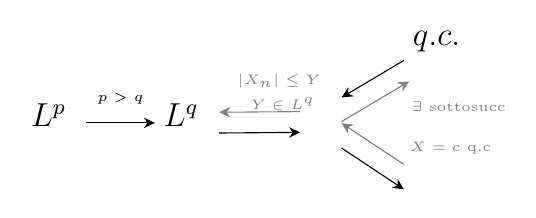
\begin{tikzpicture}[x=0.75pt,y=0.75pt,yscale=-1,xscale=1]
%uncomment if require: \path (0,119); %set diagram left start at 0, and has height of 119

% Text Node
\draw (14,50.4) node [anchor=north west][inner sep=0.75pt]  [font=\large]  {$L^{p}$};
% Text Node
\draw (78,50.4) node [anchor=north west][inner sep=0.75pt]  [font=\large]  {$L^{q}$};
% Text Node
\draw (148,50.9) node [anchor=north west][inner sep=0.75pt]  [font=\large]  {$\PP$};
% Text Node
\draw (198,85.4) node [anchor=north west][inner sep=0.75pt]  [font=\large]  {$\Lc$};
% Text Node
\draw (198,15.4) node [anchor=north west][inner sep=0.75pt]  [font=\large]  {$\text{q.c.}$};
% Text Node
\draw (46,45.4) node [anchor=north west][inner sep=0.75pt]  [font=\tiny]  {$p>q$};
% Text Node
\draw (107,32.9) node [anchor=north west][inner sep=0.75pt]  [font=\tiny,color={rgb, 255:red, 128; green, 128; blue, 128 }  ,opacity=1 ]  {$ \begin{array}{l}
| X_{n}| \leq Y\\
\ \ Y\in L^{q}
\end{array}$};
% Text Node
\draw (197.5,49.5) node [anchor=north west][inner sep=0.75pt]  [font=\tiny,color={rgb, 255:red, 128; green, 128; blue, 128 }  ,opacity=1 ] [align=left] {$\exists $ sottosucc};
% Text Node
\draw (196.5,69) node [anchor=north west][inner sep=0.75pt]  [font=\tiny,color={rgb, 255:red, 128; green, 128; blue, 128 }  ,opacity=1 ] [align=left] {$X=c$ q.c};
% Connection
\draw    (42,61) -- (72,61) ;
\draw [shift={(75,61)}, rotate = 180] [fill={rgb, 255:red, 0; green, 0; blue, 0 }  ][line width=0.08]  [draw opacity=0] (5.36,-2.57) -- (0,0) -- (5.36,2.57) -- (3.56,0) -- cycle    ;
% Connection
\draw [color={rgb, 255:red, 128; green, 128; blue, 128 }  ,draw opacity=1 ]   (109,55.86) -- (145,55.58) ;
\draw [shift={(106,55.88)}, rotate = 359.56] [fill={rgb, 255:red, 128; green, 128; blue, 128 }  ,fill opacity=1 ][line width=0.08]  [draw opacity=0] (5.36,-2.57) -- (0,0) -- (5.36,2.57) -- (3.56,0) -- cycle    ;
% Connection
\draw [color={rgb, 255:red, 0; green, 0; blue, 0 }  ,draw opacity=1 ]   (142,65.6) -- (106,65.88) ;
\draw [shift={(145,65.58)}, rotate = 179.56] [fill={rgb, 255:red, 0; green, 0; blue, 0 }  ,fill opacity=1 ][line width=0.08]  [draw opacity=0] (5.36,-2.57) -- (0,0) -- (5.36,2.57) -- (3.56,0) -- cycle    ;
% Connection
\draw    (167.58,47.2) -- (195,30.89) ;
\draw [shift={(165,48.73)}, rotate = 329.25] [fill={rgb, 255:red, 0; green, 0; blue, 0 }  ][line width=0.08]  [draw opacity=0] (5.36,-2.57) -- (0,0) -- (5.36,2.57) -- (3.56,0) -- cycle    ;
% Connection
\draw [color={rgb, 255:red, 128; green, 128; blue, 128 }  ,draw opacity=1 ]   (194.98,42.53) -- (165,60.37) ;
\draw [shift={(197.56,41)}, rotate = 149.25] [fill={rgb, 255:red, 128; green, 128; blue, 128 }  ,fill opacity=1 ][line width=0.08]  [draw opacity=0] (5.36,-2.57) -- (0,0) -- (5.36,2.57) -- (3.56,0) -- cycle    ;
% Connection
\draw [color={rgb, 255:red, 128; green, 128; blue, 128 }  ,draw opacity=1 ]   (167.5,62.79) -- (195,81.04) ;
\draw [shift={(165,61.13)}, rotate = 33.56] [fill={rgb, 255:red, 128; green, 128; blue, 128 }  ,fill opacity=1 ][line width=0.08]  [draw opacity=0] (5.36,-2.57) -- (0,0) -- (5.36,2.57) -- (3.56,0) -- cycle    ;
% Connection
\draw    (192.5,91.38) -- (165,73.13) ;
\draw [shift={(195,93.04)}, rotate = 213.56] [fill={rgb, 255:red, 0; green, 0; blue, 0 }  ][line width=0.08]  [draw opacity=0] (5.36,-2.57) -- (0,0) -- (5.36,2.57) -- (3.56,0) -- cycle    ;

\end{tikzpicture}

\subsection{Altre proprietà e teorema di Slutsky}

Dati $X_n\xrightarrow{\Lc}X,Y_n\xrightarrow{\Lc} c\in\RR,a\in\RR,h\in\Cc^0(\RR)$:\\
$\triangleright\,X_n\xrightarrow{\PP}X\Rightarrow X_n\xrightarrow{\Lc} X$ \\
$\triangleright\,X_n\xrightarrow{\Lc}c\Rightarrow X_n\xrightarrow{\PP}c\ (c\in\RR)$ \\
$\triangleright\,aX_n\xrightarrow{\PP} aX$ \\
$\triangleright\,h(X_n)\xrightarrow{\PP} h(X)$ \\
$\triangleright\,\text{Slutsky }
\begin{cases}
X_n+Y_n\xrightarrow{\Lc} X+c \\
X_nY_n\xrightarrow{\Lc} +cx \\
\frac{X_n}{Y_n(\neq 0)}\xrightarrow{\Lc} \frac{X}{c(\neq 0)}
\end{cases}$

\subsection{Proprietà generali media campionaria}

Date $X_1,\ldots,X_n$ iid si ha: \\
$\EE\left[\Xn\right]=\EE[X]$ \\
$\Var\left(\Xn\right)=\Var(X)/n$ \\
$\EE\left[\Xn^2\right]=\Var(X)/n-\EE[X]^2$

\subsection{LGN}

Date $X_i\in L^1$ iid si ha:
\begin{equation*}
\EE\left[\Xn\right]=\mu\in\RR\ \Longleftrightarrow\ \Xn\xrightarrow{\text{qc},\PP,L^1}\mu
\end{equation*}
(è utile per verificare la proprietà di consistenza di uno stimatore tipo $\hat{\theta}_{\text{MLE}}=\Xn$, senza passare per il toerema apposito)

\subsection{TCL}

Date $X_i\in L^2$ iid si ha:
\begin{gather*}
\frac{\Xn-\EE[X]}{\sqrt{\Var(X)/n}}\xrightarrow{\Lc}\Nc(0,1) \quad \text{ovvero}\\
\sqrt{n}(\Xn-\EE[X])\xrightarrow{\Lc}\Nc(0,\Var(X))\quad\text{ovvero} \\
\Xn\approx \Nc(\EE[X],\Var(X)/n) \\
(\text{tale ris. è esatto se campione gaussiano})
\end{gather*}

Applicazioni:\\
$\begin{array}{l}
\triangleright\,\frac{\text{Bi}(n,p)-np}{\sqrt{np(1-p)}}\xrightarrow{\Lc} \Nc (0,1) \\
\quad \Rightarrow\, \text{Bi}(n,p)\overset{\underset{n\,\text{big}}{}}{\simeq}\Nc(np,np(1-p)) \\
\triangleright\,\frac{\chi^2(n)-n}{\sqrt{2n}}\xrightarrow{\Lc} \Nc (0,1) \\
\quad \Rightarrow\,\chi^2(n)\overset{\underset{n\,\text{big}}{}}{\simeq}\Nc(n,2n) \\
\triangleright\,t(n)=\frac{\Nc(0,1)}{\sqrt{\chi^2(n)/n}}\xrightarrow{\Lc} \Nc (0,1)
\end{array}$

\subsection{Proprietà as. stimatori}

Def as. correttezza: una succ di stimatori $W_n$ per $\theta$ è as. non distorta se $\EE[W_n]\xrightarrow{n}\theta$

\smallskip

Def consistenza: una succ di stimatori $W_n$ per $\theta$ è consistente se $W_n\xrightarrow{\PP}\theta$, cioè $\PP(|W_n-\theta|<\Ec)\xrightarrow{n}1$

\smallskip

Come verifico tale proprietà? \\
Se $W_n\equiv \Xn$ allora è consistente (LGN sopra) \\
Altrimenti verifico che $\text{MSE}(W_n)\xrightarrow{n} 0$ (xk la convergenza quadratica implica quella in probabilità)

\smallskip

Def as. normalità: una succ di stimatori $W_n$ per $\tau(\theta)$ è as. normale se $\sqrt{n}(W_n-\tau(\theta))\xrightarrow{\Lc}\Nc(0,\sigma^2)$, cioè $W_n\approx \Nc(\tau(\theta),\sigma^2/n)$. La qtà $\sigma^2$ è detta varianza asintotica ($\neq \lim\Var$)

\smallskip

NB: anche questa prop. è gratis se $W_n\equiv\Xn$ (TCL)

\smallskip

Teo: as. normalità $\Rightarrow$ consistenza

\begin{proof} Per Slutsky: \\
$W_n-\tau(\theta)=\frac{\sigma}{\sqrt{n}}\left(\frac{W_n-\tau(\theta)}{\sigma/\sqrt{n}}\right)\xrightarrow{\Lc}0\cdot\Nc(0,1)=0$ \\
e dato che la conv. in $\Lc$ ad una cost implica quella in prob si ottiene la tesi: $W_n\xrightarrow{\PP}\tau(\theta)\quad\blacksquare$
\end{proof}

Def as. efficienza: una succ di stimatori $W_n$ per $\tau(\theta)$ è as. efficiente se $\sqrt{n}(W_n-\tau(\theta))\xrightarrow{\Lc}\Nc(0,v(\theta))$ con $v=\left(\tau'\right)^2/I_1$, cioè $W_n\approx \Nc(\tau(\theta),l_{\text{CR}})$

\smallskip

Confronto: più la var as. è piccola, più lo stimatore è eff.

\subsection{Risultati per MLE}

Sotto le ipotesi di regolarità della dis. di CR (nella pratica $\theta\notin\text{supp}X_i$) gli MLE sono: \\
$\begin{array}{l}
1)\,\text{(almeno) as. non distorti} \\
2)\,\text{consistenti} \\
3)\,\text{as. normali ed efficienti, cioè} \\
\qquad \sqrt{n}(\hat{\theta}-\theta)\xrightarrow{\Lc}\Nc(0,1/I_1) \\
\end{array}$

Ciò vale anche per $\tau(\theta)$, e la 3 diventa: \\
$\begin{array}{l}
\qquad \sqrt{n}(\tau(\hat{\theta})-\tau(\theta))\xrightarrow{\Lc}\Nc(0,v)
\end{array}$

\subsection{Metodi delta}

Delta 1: siano $W_n$ tc $\sqrt{n}(W_n-\theta)\xrightarrow{\Lc}\Nc(0,\sigma^2)$ e $g$ funz. tc $\exists g'(\theta)\neq 0$, allora: \\
$\begin{array}{c}
\sqrt{n}(g(W_n)-g(\theta))\xrightarrow{\Lc}\Nc(0,\sigma^2\cdot\left(g'(\theta)\right)^2)
\end{array}$

\smallskip

Applicato a $\Xn$ $(\mu=\EE[X]),\sigma^2=\Var(X)$: \\
$\begin{array}{l}
\sqrt{n}(g(\Xn)-g(\mu))\xrightarrow{\Lc}\Nc(0,\sigma^2\,\left(g'(\mu)\right)^2)
\end{array}$

\smallskip

Delta 2: siano $W_n$ tc $\sqrt{n}(W_n-\theta)\xrightarrow{\Lc}\Nc(0,\sigma^2)$ e $g$ funz. tc $\exists g'(\theta)$, $\exists g''(\theta)\neq 0$, allora: \\
$\begin{array}{l}
n(g(W_n)-g(\theta))\xrightarrow{\Lc} \frac{\sigma^2}{2}\,g''(\theta)\,\chi^2_1
\end{array}$

\subsection{Intervalli di confidenza asintotici}

Capiamo tutto da un esempio: $X_i\overset{\text{iid}}{\sim}f(x,\theta)$ ($\theta$ non nel supporto), trovo $\hat{\theta}_{\text{L}}$. Allora so che $\hat{\theta}_{\text{L}}$ è as. non distorto, consistente, as. normale. Per capire con che legge calcolo $I_1$ e risulta pari a $\theta^{-2}$. Allora \\
$\text{}\qquad \sqrt{n}\left(\hat{\theta}_{\text{L}}-\theta\right)\xrightarrow{\Lc}\Nc(0,\theta^2)$ \\
cioè $\hat{\theta}_{\text{L}}\approx\Nc(\theta,\theta^2/n)$.

\smallskip

Ora mi chiedo: che legge asintotica ha $\tau(\theta)=e^{-\theta}$? Con il metodo delta 1 posso subito dire che \\
$\text{}\qquad \hat{\tau}_{\text{L}}\approx\Nc\left(e^{-\theta},\frac{\theta^2}{n}\cdot e^{-2\theta}\right)$

\smallskip

Allora, se il campione è numeroso: \\
$\text{}\quad \tau(\theta)=e^{-\theta}\in\left[e^{-\hat{\theta}_{\text{L}}}\pm z_{1-\frac{\alpha}{2}}\sqrt{\frac{\hat{\theta}_{\text{L}}^2}{n}\,e^{-2\hat{\theta}_{\text{L}}}} \right]$

\smallskip

Teo: considero test $H_0:\ \theta=\theta_0$ vs $H_1:\ \theta\neq\theta_0$ e $X_1,\ldots,X_n\sim f(x,\theta)\in\text{EF}$. Allora sotto $H_0$ vale che $W=-2\log(\lambda(\xv))\xrightarrow{\Lc}\chi^2_1$

\begin{proof}
Per le prop dei logaritmi $W=2l(\xv,\hat{\theta}_L)-2l(\xv,\theta_0)$. Inoltre, per Taylor al second'ordine $l(\xv,\theta_0)=l(\xv,\hat{\theta}_L)+\cancel{ l'(\xv,\hat{\theta}_L) }(\hat{\theta}_L-\theta_0)+\frac{1}{2}l''(\xv,\hat{\theta}_L)(\hat{\theta}_L-\theta_0)^2$. Dunque $W=-l''(\xv,\hat{\theta}_L)(\hat{\theta}_L-\theta_0)^2$. Sfruttando che $I_n(\hat{\theta}_L)=-l''(\xv,\hat{\theta}_L)$ e $\frac{I_n(\hat{\theta}_L)}{n}\xrightarrow{\text{qc},\PP} I(\theta)$, sotto $H_0$ vale
$\begin{array}{l}
W=-\underbrace{l''(\xv,\hat{\theta}_L)\cdot\frac{1}{nI(\theta_0)}}_{\xrightarrow{\Lc}1} \underbrace{\left(\frac{\sqrt{n}(\hat{\theta}_L-\theta_0)}{1/\sqrt{I(\theta_0)}}\right)^2}_{\xrightarrow{\Lc}\chi^2_1}\ \blacksquare
\end{array}$
\end{proof}

% =================================================

\section{Risultati notevoli}

% =================================================

\subsection{Varianza campionaria}

${\renewcommand*{\arraystretch}{1.5}\begin{array}{l}
S^2 =\frac{1}{n-1}\sum^n_{k=1}( X_k -\overline{X}_n)^2 \\
\quad=\frac{n}{n-1}\left[\frac{\sum X_i^2}{n}-\left(\frac{\sum X_i}{n}\right)^2\right] \\
\EE\left[ S^2\right] =\sigma^2 \qquad S^2\Bot\Xn \\
S^2\xrightarrow{\text{qc}} \sigma^2\text{ analogo alla LGN per }\Xn \\
\end{array}}$

\subsection{Quantili di una gamma}

$Y\sim\Gamma(n,\lambda)\ \Rightarrow\ 2\lambda Y\sim\Gamma(n,\frac{n}{2})=\chi^2(2n)$ \\
$\text{}\ \Rightarrow\ \gamma_{1-\alpha}(n,\lambda)=x^2_{1-\alpha}(2n)/2\lambda$

% =================================================

\section{Regressione}

% =================================================

\subsection{Modello e GOF}

Forma compatta: $\yev=\ZZ\bev+\erv$

$R^2,\ R^2_{\text{adj}}$, metodi stepwise (con test F) per selezionare covariate, $VIF_j=\frac{1}{1-R^2_j}$ (per verificare la colinearità tra le covariate), plot dei leverages, plot dei residui, influential plot ...

\subsection{Stimatori OLS}

Def: $\widehat{\bev}_{\text{LS}}=\underset{\bbv\in\RR^{r+1}}{\ArgMin}\left(\yev-\ZZ\bbv\right)^T\left(\yev-\ZZ\bbv\right)$

\smallskip

Teo 1: $\widehat{\bev}_{\text{LS}}=\left(\ZZ^T\ZZ\right)^{-1}\ZZ^T\yev$

\smallskip

Teo 2: $\EE\left[\widehat{\bev}_{\text{LS}}\right]=\bev$ (stim. non distorti)

\begin{proof}
$\EE\left[\widehat{\bev}_{\text{LS}}\right]=\EE\left[\left(\ZZ^T\ZZ\right)^{-1}\ZZ^T\yev\right]$ \\
$\text{}\quad=\left(\ZZ^T\ZZ\right)^{-1}\ZZ^T\EE\left[\yev\right]$ \\
$\text{}\quad=\left(\ZZ^T\ZZ\right)^{-1}\ZZ^T\EE\left[\ZZ\bev+\erv\right]$ \\
$\text{}\quad=\left(\ZZ^T\ZZ\right)^{-1}\ZZ^T\ZZ\bev=\bev\qquad\blacksquare$ \\
\end{proof}

Teo 3: $\Cov\left(\widehat{\bev}_{\text{LS}}\right)=\sigma^2\left(\ZZ^T\ZZ\right)^{-1}$

\subsection{Decomposizione della var}

$\begin{array}{l}
\triangleright\ \SSSS_{\text{tot}}=\sum_{i=1}^n\left(y_i-\bar{y}\right)^2 \text{ variabilità tot} \\
\triangleright\ \SSSS_{\text{reg}}=\sum_{i=1}^n\left(\hat{y}_i-\bar{\hat{y}}\right)^2 \text{ var dei fittati} \\
\triangleright\ \SSSS_{\text{res}}=\sum_{i=1}^n\left(\hat{\varepsilon}_i\right)^2 \text{ var dei residui} \\
\quad \Longrightarrow\  \SSSS_{\text{tot}}= \SSSS_{\text{reg}}+ \SSSS_{\text{res}}
\end{array}$

\subsection{Coeff di determinazione}

Qntfca la \% di var dei dati spiegata dal modello: \\
$\text{}\quad R^2=\frac{ \SSSS_{\text{reg}}}{ \SSSS_{\text{tot}}}=1-\frac{ \SSSS_{\text{res}}}{ \SSSS_{\text{tot}}}\in[0,1]$

\smallskip

Può essere aggiustato rispetto al no. di covariate: \\
$\text{}\quad R^2_{\text{adj}}=1-\frac{ \SSSS_{\text{reg}}/(n-r-1)}{ \SSSS_{\text{tot}}/(n-1)}=1-(1-R^2)\frac{n-1}{n-r-1}$

\subsection{Stimatore non distorto della varianza}

Assumendo errore gaussiano (omoschedasticità), lo stimatore non distorto della varianza dell'errore è $S^2=\frac{n\hat{\sigma}^2}{n-r-1}$ perché $n\hat{\sigma}^2=\hat{\erv}^T\hat{\erv}\sim\sigma^2\chi^2(n-r-1)\,\Rightarrow\,\EE[S^2]=\sigma^2$

\begin{proof}
$\hat{\erv}\sim\Nc(0,\sigma^2(I-H))$ e quindi $\hat{\erv}^T\frac{(I-H)^{-}}{\sigma^2}\hat{\erv}\sim\chi^2(n-r-1)$. Inoltre $H\erv=0$ e quindi $\hat{\erv}=(I-H)\hat{\erv}$. Allora: \\
$\text{}\ \chi^2_{n-r-1}\sim\hat{\erv}^T\frac{(I-H)^{-}}{\sigma^2}(I-H)\hat{\erv}=\frac{\hat{\erv}^T\hat{\erv}}{\sigma^2}\ \ \blacksquare$
\end{proof}

\subsection{IC per i beta\_j di un modello con err gauss}

$\text{ IC}_{1-\alpha}=\left[\hat{\beta}_j\pm\sqrt{S^2\text{diag}_j(\ZZ^T\ZZ^{-1})}\,t_{1-\frac{\alpha}{2}}^{n-r-1}\right]$

\subsection{Test per i parametri beta}

Costruisco il test $H_0:\ \beta_j=0$ vs $H_1:\ \beta_j\neq 0$. Sotto $H_0$ vale: \\
$\text{}\qquad T_j=\frac{\hat{\beta}_j}{\sqrt{S^2\text{diag}_j(\ZZ^T\ZZ^{-1})}}\sim t^{n-r-1}$ \\
$\text{}\qquad\Rightarrow\ \Rc=\left\{\left|T_j\right|>t_{1-\frac{\alpha}{2}}^{n-r-1}\right\}$

\smallskip

\textbf{ANOVA} È un test che serve per confrontare le medie dei gruppi all'interno di un modello lineare in cui le covariate sono categoriche. Richiede che i residui siano normali e omoschedastici.

\smallskip

\textbf{Modelli lineari generalizzati} Servono per estendere i modelli lineari ai casi in gui la variabile indipendente $Y$ non è necessariamente gaussiana, ma appartiene alla EF. Bisogna specificare: la legge di $Y$, la matrice dei predittori $\ZZ$ e la link function $g(\cdot)$ ovvero quale funzione di $\EE[Y]$ si vuole modellare.

\smallskip

\textbf{Modello di regressione logistica} La random component è $Y\sim\Be(p_i)$ e la link function è quella canonica: $\text{logit}(p)=\log\left(\frac{p_i}{1-p_i}\right)=\nu_i=\beta_0+\beta_1z_{ij}+..+\beta_rz_{ir}$. Dunque $p_i=\frac{e^{\nu_i}}{1+e^{\nu_i}}$ e le stime dei coeff non sono altro che l'odds-ratio relativo alla cov $j$-esima: $\text{OR}_j=e^{\beta_j}$.

\smallskip

\textbf{Curva ROC per classificatori binari} Grafico in cui $x$ è 1-specificità e $y$ è sensibilità












